\documentclass{beamer}
\usepackage[spanish,es-noquoting]{babel}
\usepackage[utf8]{inputenc}
\usepackage[sc]{mathpazo}    % Palatino with smallcaps
\usepackage[scaled]{helvet}  % Helvetica, scaled 95%
\usepackage{eulervm}% Euler math
\usepackage{amsthm,amssymb,amsfonts,latexsym}
\usepackage{amsmath}
%\usepackage{ccfonts}
\usepackage{empheq}
\usepackage{xcolor}
\usepackage[most]{tcolorbox}
%\usepackage{textcomp}
\setbeamertemplate{theorems}[numbered]
\usepackage{ragged2e}
\usetheme[]{Darmstadt} 

\setbeamercolor{beaver}{fg=blue!90!black}
%\usecolortheme{beaver}

\newtheorem{defi}{Definición}[section]
\newtheorem{theo}[defi]{Teorema}
\newtheorem{lem}[defi]{Lema}
\newtheorem{hip}[defi]{Hipótesis}
\newtheorem{corolary}[defi]{Corolario}
\usepackage{breqn}

%\useoutertheme{shadow}
\useinnertheme{circles}
\setbeamertemplate{bibliography item}{\insertbiblabel}
\setbeamertemplate{headline}{}
\usepackage{nicefrac}

%\usepackage[demo]{graphicx}% remove demo option in actual document
\setbeamertemplate{navigation symbols}{}

\addtobeamertemplate{navigation symbols}{}{%
    \usebeamerfont{footline}%
    \usebeamercolor[fg]{footline}%
    \hspace{1em}%
}
\setbeamertemplate{caption}[numbered]
\addtobeamertemplate{block begin}{}{\justifying}


\title[Potencial Gravitacional de Yukawa en Gravedad $f(R)$]{Potencial Gravitacional de Yukawa en Gravedad $f(R)$}
\author[Julián Jiménez-Cárdenas]{Julián Jiménez-Cárdenas}
\institute{Universidad Nacional de Colombia, Bogotá. \and \texttt{juojimenezca@unal.edu.co}}
\date{}

\begin{document}
\justifying
	\frame{\titlepage}
	\frame[allowframebreaks]{\tableofcontents}
	\section{Introducción}
	\begin{frame}{Modificación de la ley de Newton}
		Una manera de aproximarse al problema de la materia y energía oscura es a través de una modificación de la ley de Newton. Tal modificación surge en el límite de campo débil de algunos modelos de gravedad.
		
		\begin{block}{Modificación de Yukawa}
						Generalización de la acción de Einstein-Hilbert:
			\begin{equation}
				S=\frac{1}{2\kappa}\int f(R)\sqrt{-g}d^4x
			\end{equation}
			$g=det(g_{\mu\nu}), \kappa=8\pi Gc^{-4}$. En el límite de campo débil, el potencial modificado de Newton toma la forma\cite{Capozziello}
			\begin{equation}
				\Phi (r)=-\frac{GM}{(1+\delta)r}(1+\delta e^{-r/\lambda})
			\end{equation}			
		\end{block}
	\end{frame}
	
	\begin{frame}{Modificación de Yukawa}
		Donde $\delta$ es la corrección de Yukawa y $\lambda$ es la escala a la cual la fuerza de Yukawa actúa.
		\begin{equation}\tag{Longitud de onda de Compton\cite{Lee}}
			\lambda=\lambda_c=\frac{hc}{m_g}
		\end{equation}
		
		\begin{block}{Parámetros de Yukawa y el Lagrangiano $f(R)$ \cite{Capozziello2}}
		\begin{equation*}
		\delta=\frac{df(R)}{dR}\Bigg|_{R=R_0}-1, \hspace{0.5cm} \lambda=\sqrt{-6\frac{d^2f(R)}{dR^2}\Bigg|_{R=R_0}\Bigg( \frac{df(R)}{dR}\Bigg|_{R=R_0} \Bigg)^{-1}}
		\end{equation*}
		
		\end{block}
	\end{frame}
	
	\section{Acercamiento Newtoniano al problema de dos cuerpos bajo el potencial de Yukawa}
	\begin{frame}{Ecuaciones del Movimiento y Energía total}
	\begin{block}{Ecuaciones del Movimiento}
	En coordenadas polares, $(r, \varphi)$, y con respecto al centro de masa, las ecuaciones del movimiento son
		\begin{equation}
		\ddot{r}-r\dot{\varphi}^2=-\frac{\partial \Phi(r)}{\partial r}
		\end{equation}
	
		\begin{equation}
		\frac{d}{dt}(r^2 \dot{\varphi})=0
		\end{equation}
	\end{block}
	
	\begin{block}{Energía Total}
		\begin{equation}
			E_T=\frac{1}{2}\mu(\dot{r}^2+r^2\dot{\varphi}^2)-\frac{GMm}{(1+\delta)r}(1+\delta e^{-r/\lambda})
		\end{equation}
		donde $\mu=\frac{Mm}{m+M}$ es la masa reducida.
	\end{block}
	\end{frame}
	
	\begin{frame}{Conservación del momento angular en la Energía}
	
	Se puede usar el momento angular del sistema para reescribir la energía total.
	
	$$E_T=\frac{1}{2}\mu\dot{r}^2+\textcolor{red}{\frac{L^2}{2\mu r^2}-\frac{GMm}{(1+\delta)}\frac{(1+\delta e^{-r/\lambda})}{r}}$$	
	
	\end{frame}
	
	\begin{frame}{Potencial efectivo}
	\begin{block}{Potencial efectivo}
		\begin{equation}
			V_{eff}(r):=\frac{L^2}{2\mu r^2}-\frac{GMm}{(1+\delta)r}-\frac{GMm\delta e^{-r/\lambda}}{(1+\delta)r}
		\end{equation}
		Algunas consideraciones sobre el potencial efectivo son las siguientes:
		\begin{itemize}
			\item $\delta\neq -1.$
			\item Si $\delta$ toma valores negativos, el segundo término permanece atractivo mientras $\delta<-1$, y el último término se vuelve repulsivo.
			\item Si $\delta<-1$, el segundo término se vuelve repulsivo y el tercer término sigue atractivo.
			\item Si $\delta>0$, el segundo y tercer término son atractivos.
		\end{itemize}
	\end{block}
	\end{frame}
	
	\begin{frame}{Potencial modificado de Newton}
		\begin{figure}
			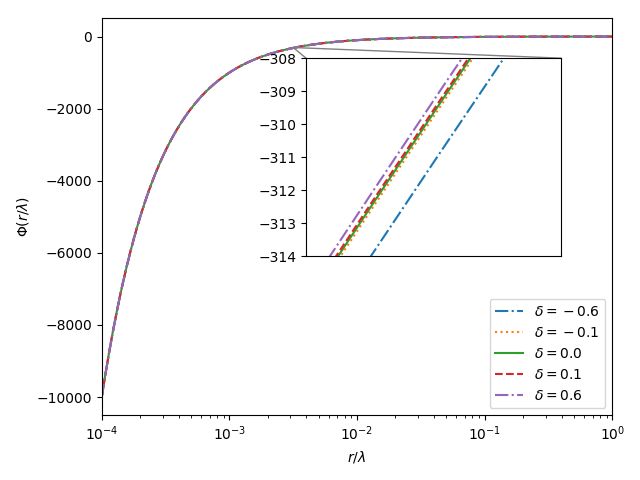
\includegraphics[width=.6\textwidth]{potential.png}
			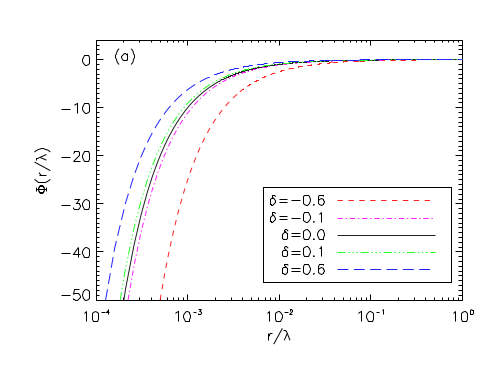
\includegraphics[width=.5\textwidth]{ar1.png}
			\caption{De derecha a izquierda: Recreación del potencial modificado de Newton en Python y figura 1 en \cite{main}.}
		\end{figure}
	\end{frame}
	
	\begin{frame}{Potencial efectivo}
	\begin{figure}
			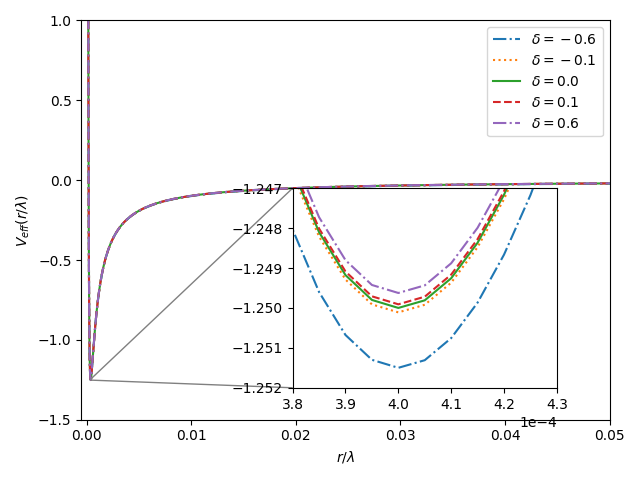
\includegraphics[width=.6\textwidth]{veff.png}
			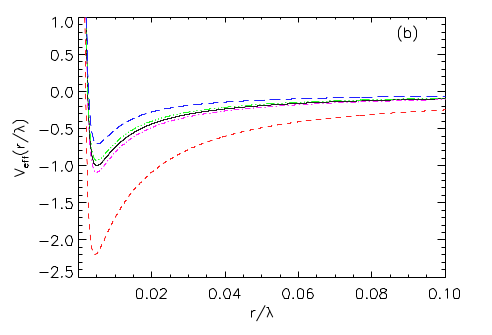
\includegraphics[width=.5\textwidth]{ar2.png}
			\caption{De derecha a izquierda: Recreación del potencial efectivo en Python y figura 1 en \cite{main}.}
			\end{figure}
	\end{frame}
	
	\begin{frame}[allowframebreaks]{Mínimo del potencial efectivo}
	Si se deriva la expresión del potencial efectivo y se iguala a cero para hallar los puntos críticos de esta función, se obtiene la expresión
	
	\begin{equation}
	\frac{L^2}{\mu r_{crit}^3}=\frac{GMm(\delta e^{-r_{crit}/\lambda}+1)}{\delta+1}+\frac{\delta GMme^{-r_{crit}/\lambda}}{(1+\delta)\lambda}r_{crit}.
	\end{equation}
	La segunda derivada da
	\begin{dmath}
	\frac{d^2V_{eff}(r)}{dr^2}=\frac{3L^2}{\mu r^4}-\frac{2GMm}{(1+\delta)r^3}(1+\delta e^{-r/\lambda})-\frac{2GMm\delta e^{-r/\lambda}}{\lambda (1+\delta)r^2}-\frac{GMm\delta e^{-r/\lambda}}{\lambda^2 (1+\delta)r}.
	\end{dmath}
	Evaluando esta última expresión en $r=r_{cri}$ y usando la expresión que determina $r_{min}$, se simplifica la forma de la segunda derivada
	\begin{equation}
	\frac{d^2V_{eff}(r)}{dr^2}\Bigg|_{r=r_{crit}}=\frac{GMme^{-r_{crit}/\lambda}}{(\delta+1)r_{crit}^3}\Bigg[\delta\Big(1+\frac{r_{crit}}{\lambda}-\frac{r_{crit}^2}{\lambda^2} \Big)+e^{r_{crit}/\lambda} \Bigg]
	\end{equation}
	Para garantizar que este punto crítico es efectivamente un mínimo en el potencial, debe ocurrir que
	\begin{equation}
	g(x)\equiv \frac{\delta(1+x-x^2)+e^x}{\delta+1}>0,
	\end{equation}
	con $x=r_{crit}/\lambda.$
	
	\begin{figure}
	\centering
	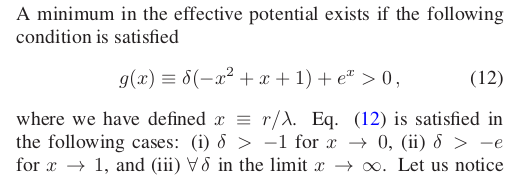
\includegraphics[width=.7\textwidth]{ar3.png}
	\caption{Definición de $g(x)$ en \cite{main}.}
	\end{figure}
	\end{frame}
	
	\begin{frame}[allowframebreaks]{$r<<\lambda, x\rightarrow 0$}
	El caso en el que $r<</\lambda$ es la configuración común de un sistema astrofísico cuya dinámica ocurre a escalas menores que la longitud de onda del gravitón. Es posible expandir la exponencial en series de potencias:
	
	\begin{equation}
		e^{\pm x}\approx 1\pm x +\frac{x^2}{2}+O(x^3)
	\end{equation}
	Reemplazando esta aproximación en el potencial $\Phi(r)$, se obtiene
	\begin{equation}
		\Phi(r)=-\frac{GM}{r}+\frac{GM\delta}{\lambda(1+\delta)}+\frac{GM\delta r}{2\lambda^2(1+\delta)}.
	\end{equation}
	El primer término es el potencial Newtoniano, el segundo un corrimiento en la energía.
	\begin{block}{Quinta fuerza}
		El tercer término genera una aceleración radial constante, que se puede escribir como
		
		$$a_{corr}=-\frac{a^*\delta}{2(1+\delta)}\frac{{r^*}^2}{\lambda^2}$$
		donde $a^*$ es la aceleración Newtoniana de un objeto a una distancia $r^*$.
	\end{block}
	El mínimo (en caso de que $g(x)>0$) para los órdenes $O(x^2)$ y $O(x^3)$ se puede calcular explícitamente, bajo la condición de que
	$$\frac{dV(r)}{dr}\Bigg|_{r=r_{min}}=0.$$
	
	\begin{block}{$O(x^2)$}
	\begin{equation}
		V_{eff}(r)=\frac{L^2}{2\mu r^2}-\frac{GMm}{(1+\delta)r}-\frac{GMm\delta}{(1+\delta)r}\Big( 1-\frac{r}{\lambda}\Big),
	\end{equation}
	
	\begin{equation}
	r_{min}=\frac{L^2}{\mu GMm}.
	\end{equation}
	El mínimo coincide con el del potencial efectivo, y su valor está corrido respecto al del potencial efectivo Newtoniano:
	\begin{equation}
		V_{eff}(r_{min})=-\frac{GMm}{2}\Bigg(\frac{G\mu Mm}{L^2}-\frac{2\delta}{\lambda(1+\delta)}\Bigg).
	\end{equation}
	\end{block}
	
	\begin{block}{$O(x^3)$}
	\begin{equation}
	V_{eff}(r)=\frac{L^2}{2\mu r^2}-\frac{GMm}{r}+\frac{\delta GMm}{\lambda(1+\delta)}-\frac{\delta GMmr}{2(\delta+1)\lambda^2}.
	\end{equation}
	Cuando se deriva el último término, que va como $\delta/\lambda^2$, debido a que se trabaja con el régimen  $\delta<<1$ (pequeñas desviaciones del caso Newtoniano), el corrimiento de $r_{min}$ es despreciable.
	
	El potencial efectivo es en este punto:
	\begin{equation}
		V_{eff}(r_{min})=-\frac{GMm}{2}\Bigg(\frac{G\mu Mm}{L^2}-\frac{2\delta}{\lambda(1+\delta)}\Bigg)-\frac{L^2\delta}{2(1+\delta)\lambda^2\mu}.
	\end{equation}
	\end{block}
	\end{frame}
	
	\section{Ecuaciones de las órbitas}
	\subsection{Aproximación a orden $O(x^2)$}
	\begin{frame}[allowframebreaks]{Aproximación a orden $O(x^2)$}
		Se usa la conservación del momento angular para escribir
		\begin{equation}
			\dot{r}=\dot{\varphi}\frac{dr}{d\varphi}=\frac{L}{\mu r^2}\frac{dr}{d\varphi}=-\frac{L}{\mu}\frac{d}{d\varphi}\Big(\frac{1}{r} \Big).
	\end{equation}
	Entonces, a segundo orden, la energía se puede reescribir como
	\begin{block}{Energía total a segundo orden}
	\begin{equation}
		E_T=\frac{L^2}{2\mu}\Big( \frac{d}{d\varphi}\Big(\frac{1}{r}\Big) \Big)+\frac{L^2}{2\mu r^2}-\frac{GMm}{r}+\frac{\delta GMm}{(1+\delta)\lambda}.
	\end{equation}
	\end{block}
	De aquí se puede deducir la siguiente ecuación diferencial
	\begin{equation}
		(u')^2+u^2-2\beta_0 u=\beta_1
	\end{equation}
	Donde $u=1/r$, $u'=\frac{d(1/r)}{d\varphi}$ y
	\begin{equation}
	\gamma=GMm; \ \beta_0=\frac{\mu\gamma}{L^2}; \ \beta_1=\frac{2\mu E_T}{L^2}-\frac{2\mu\gamma}{L^2\lambda}\frac{\delta}{1+\delta}.
	\end{equation}
	Derivando nuevamente la ecuación diferencial, se obtiene
	\begin{equation}
		u'(u''+u-\beta_0)=0.
	\end{equation}
	Se buscan soluciones Keplerianas, dado que la energía es casi la misma que en el caso Kepleriano, de modo que se hace la suposición
	$$u\equiv \frac{1}{r}=\frac{1}{l}(1+\epsilon\cos\varphi),$$
	donde $l$ es el parámetro de la elipse y $\epsilon$ la excentricidad. Ingresando esta suposición en las ecuaciones diferenciales, se obtiene
	\begin{equation}
	l=\frac{1}{\beta_0}
	\end{equation}
	\begin{equation}
	\epsilon^2=1+l^2\beta_1
	\end{equation}
	En términos de las constantes del movimiento, la excentricidad queda como
	\begin{equation}
		\epsilon^2=1-\frac{2L^2}{\mu\gamma}\frac{\delta}{(1+\delta)\lambda}+\frac{2E_TL^2}{\mu\gamma^2}.
	\end{equation}
	Cuando $\delta=0,$ se recobra el valor Newtoniano
	$$\epsilon^2=1+\frac{2E_T L^2}{\gamma^2\mu}.$$
	
	\begin{figure}
	\centering
	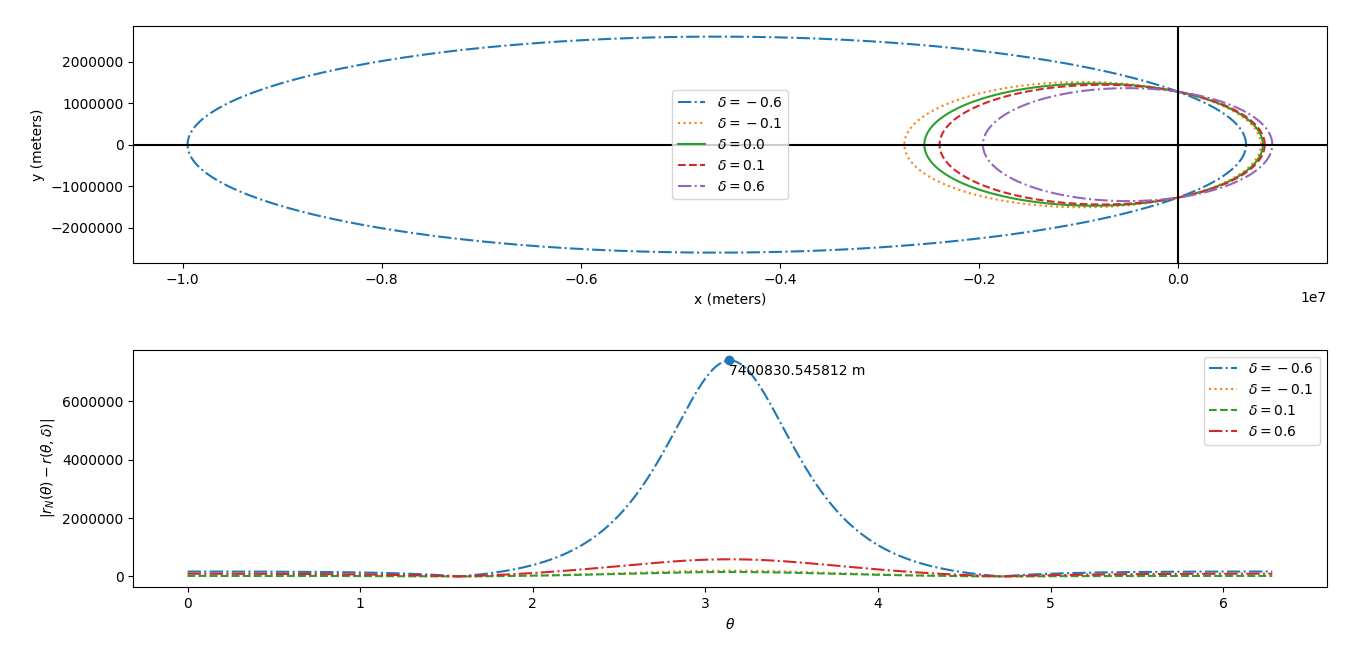
\includegraphics[width=1\textwidth]{orbits2.png}
	\caption{Ilustración del efecto del potencial gravitacional modificado sobre los parámetros orbitales.}
	\end{figure}
	
	\begin{figure}
	\centering
	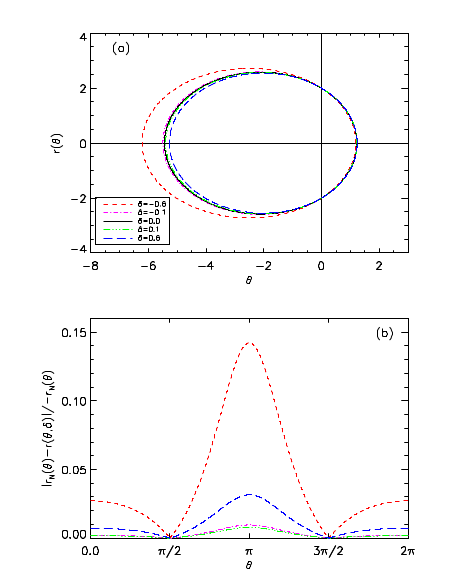
\includegraphics[width=.45\textwidth]{orbits2ref.png}
	\caption{Ilustración del efecto del potencial gravitacional modificado sobre los parámetros orbitales\cite{main}.}
	\end{figure}
	\end{frame}
	
	\subsection{Aproximación a orden $O(x^3)$}
	\begin{frame}[allowframebreaks]{Aproximación a orden $O(x^3)$}
	A tercer orden, la ecuación diferencial procedente de la energía adquiere un nuevo término
	\begin{equation}
		(u')^2+u^2-2\beta_0 u-\beta_2\frac{1}{u}=\beta_1,
	\end{equation}
	donde $\beta_0, \beta_1$ son las mismas constantes del caso anterior, y
	$$\beta_2=\frac{\mu\gamma\delta}{L^2\lambda^2(1+\delta)}$$
	Tomando la derivada de la ecuación diferencial,
	\begin{equation}
		u'(u''+u+\frac{\beta_2}{2u^2}-\beta_0)=0
	\end{equation}
	se introduce nuevamente $u\equiv 1/r=(1+\epsilon\cos\varphi)/l$, pero en este caso se evalúa para $\varphi=0,\varphi=\pi,$ obteniendo el sistema de ecuaciones diferenciales\vspace{10cm}
	\begin{block}{Sistema para $l$ y $\epsilon$}
				\begin{equation}
		\epsilon^2(1-l\beta_0)+2\epsilon(1-l\beta_0)-l\beta_0+\frac{l^3\beta_2}{2}+1=0
		\end{equation}
		\begin{equation}
		\epsilon^2(1-l\beta_0)-2\epsilon(1-l\beta_0)-l\beta_0+\frac{l^3\beta_2}{2}+1=0
		\end{equation}
	\end{block}
	Restando ambas ecuaciones, se obtiene que
	
	$$l=\frac{1}{\beta_0}.$$
	Introduciendo ahora nuestra suposición para $u$ en la primera ecuación diferencial y evaluando nuevamente, en $\varphi=0,\pi,$ se obtiene la excentricidad,
	$$\epsilon^2=1+l^2\beta_1+l^3\beta_2,$$
	
	resultado distinto al calculado en el artículo.
	\begin{figure}
	\centering
	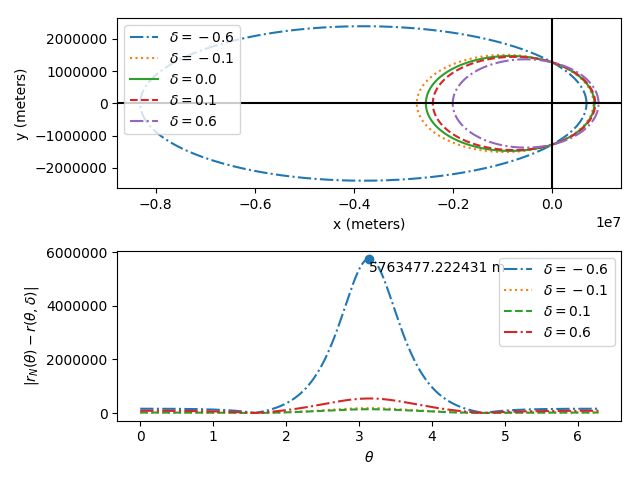
\includegraphics[width=.8\textwidth]{orbits3.png}
	\caption{Ilustración del efecto del potencial gravitacional modificado sobre los parámetros orbitales, $O(x^3)$\cite{main}.}
	\end{figure}
	\begin{figure}
	\centering
	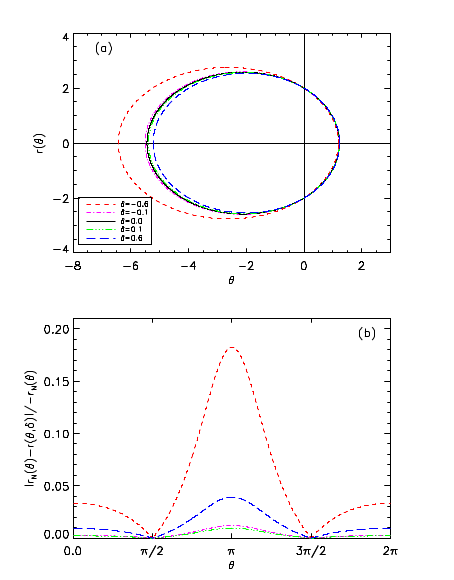
\includegraphics[width=.45\textwidth]{orbits3ref.png}
	\caption{Ilustración del efecto del potencial gravitacional modificado sobre los parámetros orbitales, $O(x^3)$\cite{main}.}
	\end{figure}
	\end{frame}	

	\section{Precesión en el Potencial de Yukawa}
	
	\begin{frame}[allowframebreaks]{Precesión en el potencial de Yukawa}
	\justifying
	Para el hallar corrimiento en el periastro debido al potencial de Yukawa, se estudian pequeñas perturbaciones de la órbita circular. Considere primero la energía total
	\begin{equation}
		(u')^2+u^2+\frac{g(u)}{L^2}=\frac{2\mu E_T}{L^2}-\frac{2\mu\gamma}{L^2\lambda}\frac{\delta}{1+\delta}
	\end{equation}
	$g(u)$ refiere a la interacción gravitacional. Se impone una órbita cerrada, con una distancia mínima y máxima al centro
	
	\begin{center}
	$r_-|_{\varphi=0}=a(1-\epsilon)$ y $r_+|_{\varphi=\pi}=a(1+\epsilon)$
	\end{center}
	$a$ es el semieje mayor de la órbita. Estos valores corresponden a 
	
	\begin{center}
		$u_0=\frac{1}{r_-}$ y $u_1=\frac{1}{r_+}$.
	\end{center}

	Al ser máximo y mínimo, se satisface que $u'|_{u=u_0}=u'|_{u=u_1}=0$. Evaluando la energía en estos puntos,
	
	\begin{empheq}[box=\tcbhighmath]{equation}
		u_0^2+\frac{g(u_0)}{L^2}=\frac{2\mu E_T}{L^2}-\frac{2\mu\gamma}{L^2\lambda}\frac{\delta}{1+\delta}
	\end{empheq}
	\begin{empheq}[box=\tcbhighmath]{equation}
	u_1^2+\frac{g(u_1)}{L^2}=\frac{2\mu E_T}{L^2}-\frac{2\mu\gamma}{L^2\lambda}\frac{\delta}{1+\delta}
	\end{empheq}
	De las cuales se obtiene que
	\tcbset{highlight math style={enhanced,colframe=red!60!black,colback=yellow!50!white,arc=4pt,boxrule=1pt,drop fuzzy shadow}}
	
	\begin{empheq}[box=\tcbhighmath]{equation}
	L^2 =\frac{g(u_0)-g(u_1)}{u_1^2-u_0^2}
	\end{empheq}
	
	\begin{empheq}[box=\tcbhighmath]{equation}
	E_T=\frac{u_1^2g(u_0)-u_0^2g(u_1)}{2\mu(u_1^2-u_0^2)}+\frac{\gamma}{\lambda}\frac{\delta}{1+\delta}
	\end{empheq}
	Despejando $u'$ en la ecuación de la energía, se obtiene
	
	\begin{equation}
		u'=\sqrt{G(u_0,u_1,u)},
	\end{equation}
	donde $G(u_0,u_1,u)$ es
	\begin{equation}
		G(u_0,u_1,u)=\frac{g(u_0)(u_1^2-u^2)+g(u_1)(u^2-u_0^2)-(u_1^2-u_0^2)g(u)}{g(u_0)-g(u_1)}.
	\end{equation}
	
	El ángulo recorrido para ir de  $r_-$ a $r_+$ será
	
	\tcbset{highlight math style={enhanced,colframe=green!60!black,colback=yellow!50!white,arc=4pt,boxrule=1pt,drop fuzzy shadow}}
	\begin{empheq}[box=\tcbhighmath]{equation}
	\varphi(r_+)-\varphi(r_-)=\int\limits_{u_0}^{u_1} G(u_0,u_1,u)^{-1/2} du
	\end{empheq}
	
	La precesión por revolución se puede ver como
	
	\begin{equation}
		\boxed{\omega=2|\varphi(r_+)-\varphi(r_-)| -2\pi}
	\end{equation}
	
	\textbf{A orden $O(x^2)$,} $g(u)=-2\mu\gamma u=2\mu\Phi_N(1/u)$, donde $\Phi_N(1/u)$ es el potencial Newtoniano. Por comparación, no hay precesión. Sin embargo, \textbf{a orden $O(x^3)$} se tiene que 
	
	$$g(u)=2\mu\Phi_N(1/u)-\frac{\mu\gamma\delta}{\lambda^2(1+\delta)}\frac{1}{u}$$
	
	Para resolver la integral que da el ángulo recorrido, se hace el cambio de variables
	
	\begin{center}
		$u_1=u_0+\eta$, $u=u_0+\eta v$, con $0<v<1.$ Así,
	\end{center}

	\begin{equation}
		\Delta \varphi \equiv \varphi(r_+)-\varphi(r_-) = \eta \int\limits_0^1 g(u_0,u_0+\eta,\lambda,\delta,u_0+\eta v) dv,
	\end{equation}
	
	donde $g(u_0,u_0+\eta,\lambda,\delta,u_0+\eta v)=\frac{1}{\sqrt{G(u_0,u_0+\eta,\lambda,\delta,u_0+\eta v)}}.$ Definiendo la variable auxiliar $\xi \equiv (1+\delta)\lambda^2.$
	\end{frame}
	% Referencias ==========================
	\section{Referencias}
	\begin{frame}[allowframebreaks]{Referencias}
	\begin{thebibliography}{9}
		\bibitem{Capozziello} S. Capozziello, M. De Laurentis, Annalen der Physik 524, 545 (2012) 
		
		\bibitem{Lee} K. Lee, F. A. Jenet, R. H. Price, N. Wex, M. Kramer Astrophys.
		
		\bibitem{Capozziello2} S. Capozziello, M. De Laurentis, Phys. Rept. 509, 167 (2011).
J. 722, 1589-1597 (2010)

		\bibitem{main} I. Martino, R. Lazkoz. Analysis of the Yukawa gravitational potential in f (R) gravity I: semiclassical periastron advance.
	\end{thebibliography}
	\end{frame}
\end{document}